% ------------------- Aufgabe a -------------------
% R1: 67,23 \pm 0,1 (ohm)
% L: 16,87 \pm 0,05 (mH)
% positver Teil Parameter für Fit % y = a*exp(-b*x):
% a pos: 3.28805437898182 in V
% b pos: 4658.956201430903 in Hz
% negativer Teil Parameter für Fit % y = -a*exp(-b*x):
% a: 3.195407081244171 in V
% b neg: 4964.215848906855 in Hz
% R_eff_exp: 162.3+/-0.5 in ohm
% ------------------- Aufgabe b -------------------
% R_ap Theo: 5723+/-9 (ohm)
% ------------------- Aufgabe c -------------------
% Resonanzüberhöhung q theo: 4.226096298726022
% delta_omega theo: (4.043+/-0.012)e+04 in Hz
% delta_freq  theo(Breite der Resonanzkurve): 6434+/-20 in Hz
% delta_freq  exp(Breite der Resonanzkurve): 9309.999999999998 in Hz
% Güte/Resonanzüberhöhung q theo: 4.196+/-0.008 in V
% Güte/Resonanzüberhöhung q exp: 3. in V
% Spannung von omega+ und omega- theo: 2.9883013507765392
% Spannung von omega+ und omega- exp: 2.220+/-0.016
% Frequenz 1 theo: 30.41+/-0.05 in kHz
% Frequenz 2 theo: 23.97+/-0.04 in kHz
% Frequenz 1 exp: 20,85 in kHz
% Frequenz 2 exp: 30.16 in kHz

\nocite{anleitungV354}
\section{Auswertung}
\label{sec:Auswertung}
Für diesen Versuch werden die folgenden Größen verwendet
 \begin{align*}
    R_1 &= (67,2 \pm 0,1) \, \unit{\ohm} \\
    R_2 &= (682 \pm 0,5) \, \unit{\ohm} \\
    R_3 &= 1 \text{ bis } 10 \, \unit{\kilo\ohm} \\
    L &= (16,87 \pm 0,05) \, \unit{\milli\henry} \\
    C &= (2,060 \pm 0,003) \, \unit{\nano\farad}\,.
\end{align*}
\\
Außerdem werden im Folgenden die Mittelwerte mit 
$$\bar{x} = \frac{1}{n} \cdot \sum_{i = 1}^{n}x_i$$ bestimmt. $n$ ist die Anzahl der Daten und $x_i$ die einzelnen Daten.
Mit der Gaußschen Fehlerfortpflanzung
$$\Delta f = \sqrt{\sum_{i = 1}^{n} \left( \frac{\partial f}{\partial x_i} \right)^2 \cdot \left(\Delta x_i \right)^2}$$
werden die Messunischerheiten ausgerechnet, wenn eine Größe von mehreren fehlerbehafteten Größen abhängt.
\subsection{Amplitude einer gedämpften Schwingung}
Bei dieser Durchführung wird der Widerstand $R_1$ verwendet.
In der Tabelle (\ref{tab:gedämpfteSchwingung}) sind die gemessenen zeitabhängigen Amplituden einer gedämpften Schwingung aufgeführt.
Hier wird, anders als im Anhang zu erkennen, der Nullpunkt der Zeit um $215\,\unit{\micro\second}$ verschoben damit die Zeiten positiv sind.
Diese Verschiebung hat allerdings keine Auswirkung auf die Zeitabhängigkeit der Amplituden. 
\begin{table}[H]
  \centering
  \caption{Gemessene Amplituden in Abhängigkeit der Zeit einer gedämpften Schwingung.}
  \label{tab:gedämpfteSchwingung}
  \begin{tblr}{colspec={c c || c c || c c}}
      \toprule
      $t\,[\unit{\micro\second}]$ & $U\,[\unit{\volt}]$ & $t\,[\unit{\micro\second}]$ & $U\,[\unit{\volt}]$ & $t\,[\unit{\micro\second}]$ & $U\,[\unit{\volt}]$\\
      \midrule
      2,50    & -3,20 & 155,00  & -1,40 & 280,00  & -1,00 \\  
      7,50    &  3,10 & 165,00  &  1,35 & 315,00  &  1,00 \\    
      47,50   & -2,40 & 200,00  & -1,30 & 325,00  & -0,40 \\  
      57,50   &  2,40 & 207,50  &  1,25 & 445,00  &  0,40 \\  
      65,00   & -2,20 & 220,00  & -1,15 & 370,00  & -0,35 \\  
      102,50  &  2,20 & 227,50  &  1,15 & 380,00  &  0,35 \\   
      110,00  & -2,05 & 237,50  & -1,10 & 387,50  & -0,30 \\  
      145,00  &  2,00 & 272,50  &  1,05 & 422,50  &  0,30 \\   
      \bottomrule
  \end{tblr}
\end{table}
Diese Messdaten sind graphisch in der Abbildung (\ref{fig:gedämpfteSchwingung}) dargestellt. Zusätzlich werden zwei exponentielle Regressionen durchgeführt.
Hierfür wird $$y = a \cdot \exp{(-b\cdot x)}$$ verwendet. 
Für die Spannungen $U > 0$ ergeben sich die Werte
\begin{align*}
  a_{\text{pos.}} &= 3,29\,\unit{\volt}\\
  b_{\text{pos.}} &= 4658,96\,\unit{\hertz}\,.
\end{align*}
Für die Spannungen $U < 0$ ergeben sich die Werte
\begin{align*}
  a_{\text{neg.}} &= -3,20\,\unit{\volt}\\
  b_{\text{neg.}} &= 4964,21\,\unit{\hertz}\,.
\end{align*}
\begin{figure}[H]
  \centering
  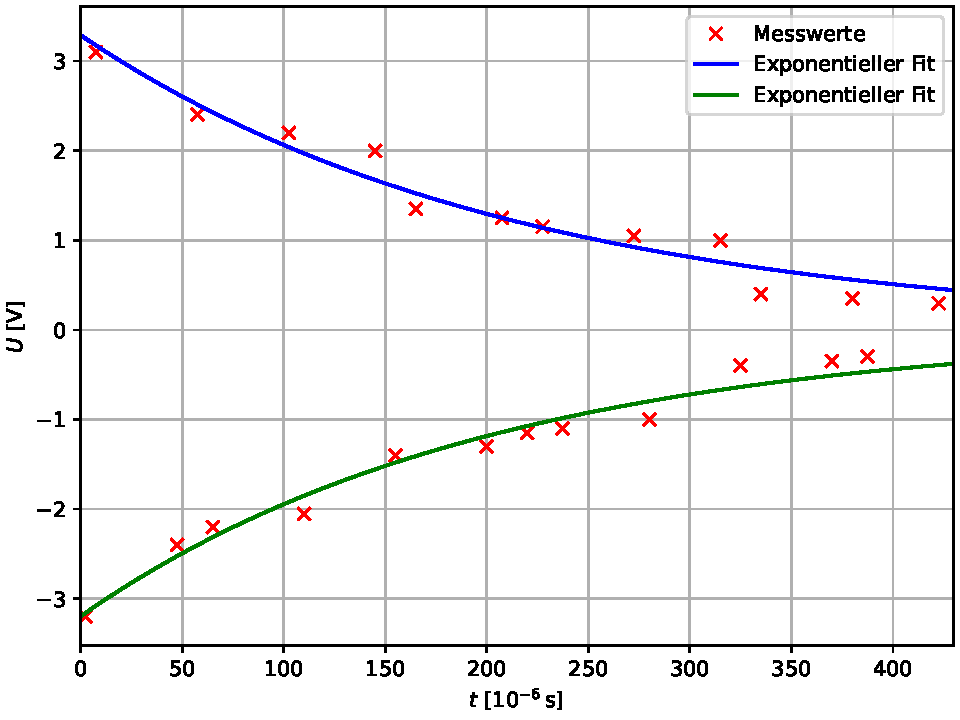
\includegraphics[width=0.90\textwidth]{plot_a.pdf}
  \caption{Zeitabhängigkeit der Spannung.}
  \label{fig:gedämpfteSchwingung}
\end{figure}
Anhand des gemittelten Werts $b = 4811,585$ aus den Werten $b_{\text{pos.}}$ und $b_{\text{neg.}}$ ergibt sich mit der Gleichung (\ref{eqn:})
der effektive Widerstand 
$$R_{\text{eff,exp.}} = 2\cdot b\cdot L = \left(162,3\pm0,5\right)\,\unit{\ohm}\,.$$
%
%
%
\subsection{Aperiodischen Grenzfall}
Mithilfe des verstellbaren Widerstands $R_3$ wird im Experiment der aperiodische Widerstand ermittelt und beträgt
$$R_{\text{ap,exp.}} = 4500\,\unit{\ohm}\,.$$
Durch Einsetzen von $L$ und $C$ in die Gleichung (\ref{eqn:}) wird der theoretische aperiodische Widerstand
$$R_{\text{ap,theo.}} = (5723\pm9)\,\unit{\ohm}\,.$$ bestimmt.
%
%
%
\subsection{Frequenzabhängigkeit der Kondensatorspannung}
Für diese Durchführung wird der Widerstand $R_2$ verwendet. Die gemessenen Spannungen in Abhängigkeit der Frequenz sind in der 
Tabelle (\ref{tab:Kondensatorspannung}) aufgeführt. Zusätzlich wird in der Tabelle (\ref{tab:Kondensatorspannung}) das Verhältnis $\frac{U}{U_0}$ festgehalten.
Hierfür wird die Spannung $U_0 = 2,15\,\unit{\volt}$ bestimmt. 
\begin{table}[H]
  \centering
  \caption{Gemessene Spannung in Abhängigkeit der Frequenz.}
  \label{tab:Kondensatorspannung}
  \begin{tblr}{colspec={c c c|| c c c}}
      \toprule
      $f\,[\unit{\kilo\hertz}]$ & $U\,[\unit{\volt}]$ & $\frac{U}{U_0}$ & $f\,[\unit{\kilo\hertz}]$ & $U\,[\unit{\volt}]$ & $\frac{U}{U_0}$\\
      \midrule
      11,03   & 2,35 & 1,093 & 26,53   & 6,75 & 3,140 \\
      13,53   & 2,50 & 1,163 & 27,03   & 6,50 & 3,023\\
      15,53   & 3,20 & 1,488 & 28,03   & 6,60 & 3,070\\
      17,53   & 2,90 & 1,349 & 28,53   & 6,40 & 2,977\\
      19,03   & 4,20 & 1,953 & 30,53   & 4,40 & 2,047\\
      20,53   & 4,50 & 2,093 & 32,03   & 4,00 & 1,860\\       
      22,53   & 6,20 & 2,884 & 33,53   & 2,60 & 1,209\\
      23,03   & 6,00 & 2,791 & 35,53   & 2,30 & 1,070\\
      24,53   & 6,50 & 3,023 & 37,53   & 2,00 & 0,930\\
      25,53   & 6,75 & 3,140 & 40,03   & 1,30 & 0,605\\
      \bottomrule
  \end{tblr}
\end{table}
In der Abbildung (\ref{fig:Frequenzabhängigkeit}) ist das Verhätnis $\frac{U}{U_0}$ gegen die Frequenz $f$ halblogarithmisch aufgetragen. 
Gleichzeitig wird mit der Gleichung (\ref{eqn:Theoriekurve}) die Theoriekurve bestimmt, die ebenfalls in der Abbildung (\ref{fig:Frequenzabhängigkeit}) 
dargestellt ist.
\begin{figure}[H]
  \centering
  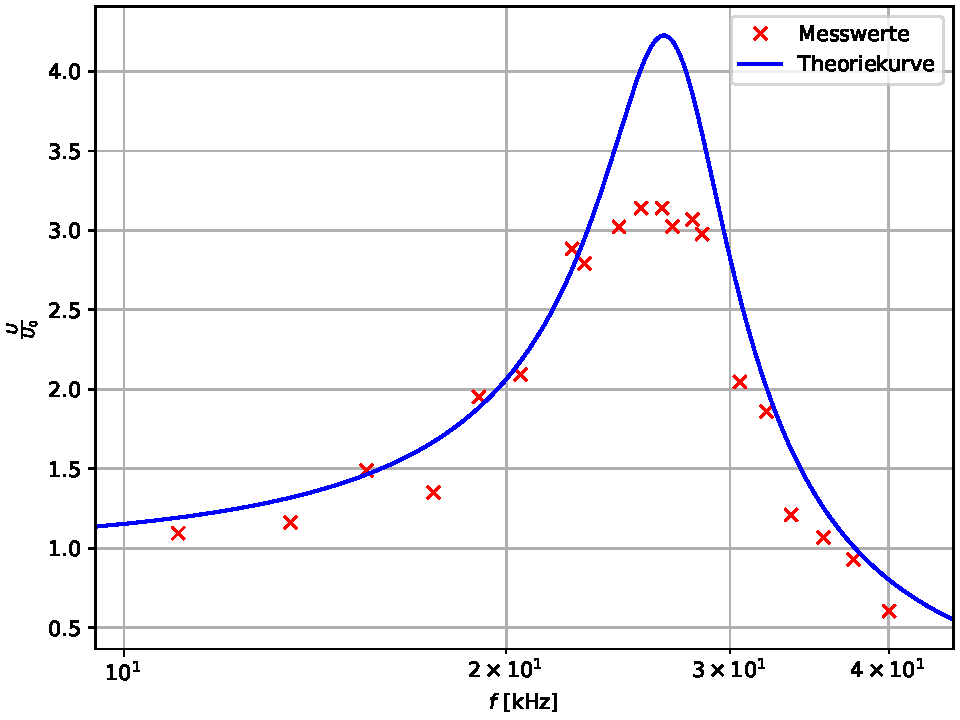
\includegraphics[width=0.90\textwidth]{plot_b.pdf}
  \caption{Frequenzabhängigkeit der Spannung und die Theoriekurve.}
  \label{fig:Frequenzabhängigkeit}
\end{figure}
Anhand der Tabelle (\ref{tab:Kondensatorspannung}) lässt sich die Resonanzüberhöhung bzw. Güte bei einer Frequenz $f = 26,53\,\unit{\kilo\hertz}$ abschätzen. Demnach ergibt sich für die 
experimentelle Güte
$$q_{\text{exp.}}= 3,140\,.$$
Die theoretische Güte wird mit den Gleichungen (\ref{eqn:BreiteResonanzkurve}) und (\ref{eqn:Güte}) bestimmt und beträgt
$$q_{\text{theo.}}=\left( 4,196\pm0,008 \right)\,.$$
Die Breite des Resonanzbereichs, wird ermittelt, indem die beiden Frequenzen bestimmt werden, bei denen das Verhältnis $\frac{U}{U_0}$ das $\frac{1}{\sqrt{2}}$-fache von der
Güte $q$ beträgt. Dafür wird in Abbildung (\ref{fig:Resonanzbereich}) ein Ausschnitt der Messwerte linear dargestellt. Anhand dieser Abbildung lässt sich ablesen
bei welchen Frequenzen $\frac{U}{U_0} = 2.220$ gilt.
Daraus ergeben sich die Frequenzen
\begin{align*}
  f_{1,\text{exp.}} &= 20,85\,\unit{\kilo\hertz}\\
  f_{2,\text{exp.}} &= 30,16\,\unit{\kilo\hertz}\,.
\end{align*}
Demnach ergibt sich für den experimentellen Resonanzbereich 
$$\Delta f_{\text{exp.}}=  f_{2,\text{exp.}}-  f_{1,\text{exp.}}= 9,31\,\unit{\kilo\hertz}\,.$$
Die theoretische Breite des Resonanzbereich wird mithilfe der Gleichung (\ref{eqn:BreiteResonanzkurve}) abgeschätzt. Somit beträgt die Breite
$$\Delta f_{\text{theo.}}= \left(6434\pm20\right)\,\unit{\hertz}\,.$$
\begin{figure}[H]
  \centering
  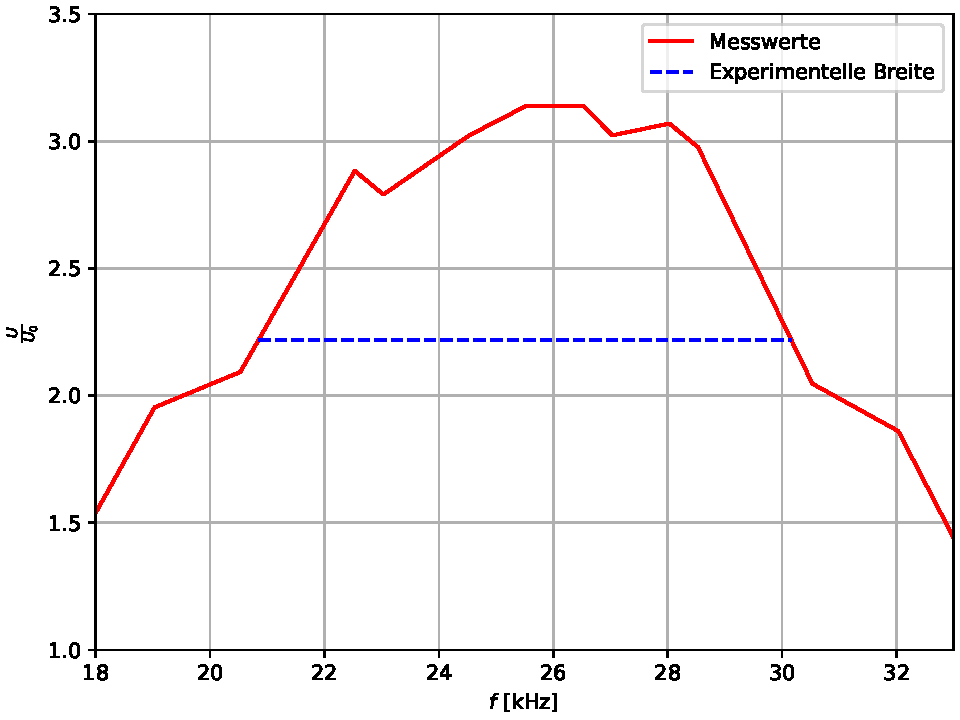
\includegraphics[width=0.90\textwidth]{plot_c.pdf}
  \caption{Linear aufgertagene Messdaten mit dem Resonanzbereich.}
  \label{fig:Resonanzbereich}
\end{figure}
% \begin{figure}
%   \centering
%   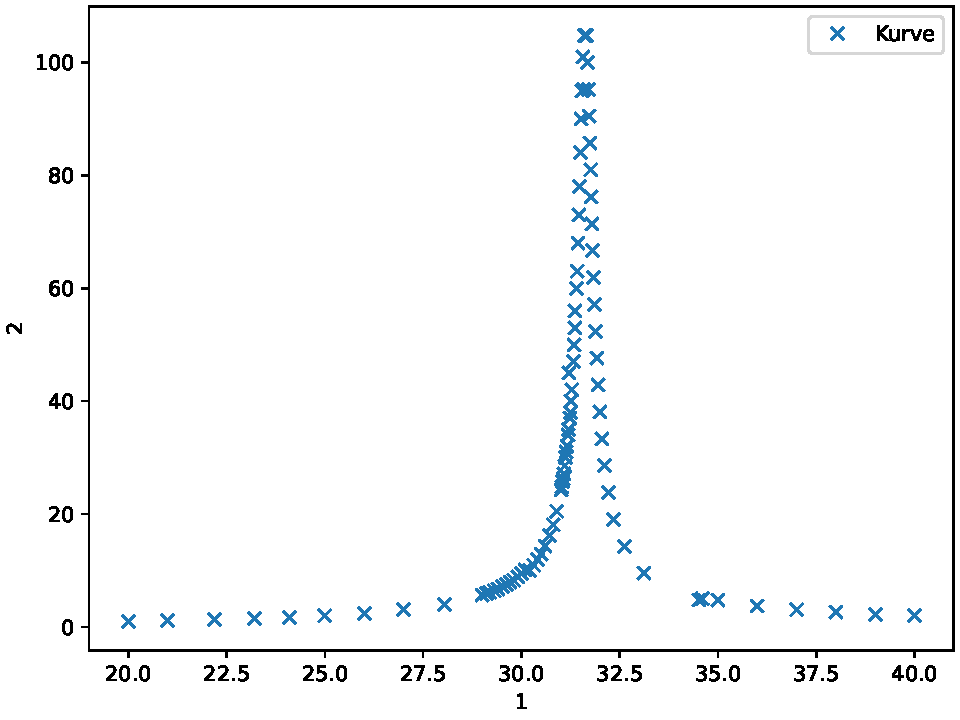
\includegraphics{plot.pdf}
%   \caption{Plot.}
%   \label{fig:plot}
% \end{figure}

%Siehe \autoref{fig:plot}!